%%%%%%%%%%%%%%%%%%%%%%%%%%%%%%%%%%%%%%%%%
% Beamer Presentation
% LaTeX Template
% Version 1.0 (10/11/12)
%
% This template has been downloaded from:
% http://www.LaTeXTemplates.com
%
% License:
% CC BY-NC-SA 3.0 (http://creativecommons.org/licenses/by-nc-sa/3.0/)
%
%%%%%%%%%%%%%%%%%%%%%%%%%%%%%%%%%%%%%%%%%

%----------------------------------------------------------------------------------------
%	PACKAGES AND THEMES
%----------------------------------------------------------------------------------------

\documentclass[UTF8,aspectratio=169,12pt]{ctexbeamer}

\usepackage{hyperref}
\hypersetup{
	colorlinks=true,
	linkcolor=red,
	anchorcolor=blue,
	citecolor=green
}

\mode<presentation> {
	
	% The Beamer class comes with a number of default slide themes
	% which change the colors and layouts of slides. Below this is a list
	% of all the themes, uncomment each in turn to see what they look like.
	
	%\usetheme{default}
	%\usetheme{AnnArbor}
	%\usetheme{Antibes}
	%\usetheme{Bergen}
	%\usetheme{Berkeley}
	%\usetheme{Berlin}
	%\usetheme{Boadilla}
	%\usetheme{CambridgeUS}
	%\usetheme{Copenhagen}
	%\usetheme{Darmstadt}
	%\usetheme{Dresden}
	%\usetheme{Frankfurt}
	%\usetheme{Goettingen}
	%\usetheme{Hannover}
	%\usetheme{Ilmenau}
	%\usetheme{JuanLesPins}
	%\usetheme{Luebeck}
	\usetheme{Madrid}
	%\usetheme{Malmoe}
	%\usetheme{Marburg}
	%\usetheme{Montpellier}
	%\usetheme{PaloAlto}
	%\usetheme{Pittsburgh}
	%\usetheme{Rochester}
	%\usetheme{Singapore}
	%\usetheme{Szeged}
	%\usetheme{Warsaw}
	
	% As well as themes, the Beamer class has a number of color themes
	% for any slide theme. Uncomment each of these in turn to see how it
	% changes the colors of your current slide theme.
	
	%\usecolortheme{albatross}
	%\usecolortheme{beaver}
	%\usecolortheme{beetle}
	%\usecolortheme{crane}
	%\usecolortheme{dolphin}
	%\usecolortheme{dove}
	%\usecolortheme{fly}
	%\usecolortheme{lily}
	%\usecolortheme{orchid}
	%\usecolortheme{rose}
	%\usecolortheme{seagull}
	%\usecolortheme{seahorse}
	%\usecolortheme{whale}
	%\usecolortheme{wolverine}
	
	%\setbeamertemplate{footline} % To remove the footer line in all slides uncomment this line
	%\setbeamertemplate{footline}[page number] % To replace the footer line in all slides with a simple slide count uncomment this line
	
	%\setbeamertemplate{navigation symbols}{} % To remove the navigation symbols from the bottom of all slides uncomment this line
}

\usepackage{graphicx} % Allows including images
\graphicspath{{./figs/}}
\usepackage{booktabs} % Allows the use of \toprule, \midrule and \bottomrule in tables
\usepackage{longtable}
\usepackage{xcolor}
\usepackage{minted}
\usepackage{listings}
\lstset{numbers=left, %设置行号位置
	numberstyle=\tiny, %设置行号大小
	keywordstyle=\color{blue}, %设置关键字颜色
	commentstyle=\color[cmyk]{1,0,1,0}, %设置注释颜色
	frame=single, %设置边框格式
	escapeinside=``, %逃逸字符(1左面的键),用于显示中文
	%breaklines, %自动折行
	extendedchars=false, %解决代码跨页时,章节标题,页眉等汉字不显示的问题
	xleftmargin=2em,xrightmargin=2em, aboveskip=1em, %设置边距
	tabsize=4, %设置tab空格数
	showspaces=false %不显示空格
}
% Fonts
% \usepackage{libertine}
% \setmonofont{Courier}
%\setCJKsansfont[ItalicFont=Noto Serif CJK SC Black, BoldFont=Noto Sans CJK SC Black]{Noto Sans CJK SC}


%----------------------------------------------------------------------------------------
%	TITLE PAGE
%----------------------------------------------------------------------------------------

\title[第16讲]{第十六讲 :进程通信} % The short title appears at the bottom of every slide, the full title is only on the title page
\subtitle{第6节:Binder机制}
\author{向勇、陈渝、李国良} % Your name
\institute[清华大学] % Your institution as it will appear on the bottom of every slide, may be shorthand to save space
{
	清华大学计算机系 \\ % Your institution for the title page
	\medskip
	\textit{xyong,yuchen,liguoliang@tsinghua.edu.cn} % Your email address
}
\date{\today} % Date, can be changed to a custom date

\begin{document}

\begin{frame}
\titlepage % Print the title page as the first slide
\end{frame}

%----------------------------------------------
%\begin{frame}
%\frametitle{提纲} % Table of contents slide, comment this block out to remove it
%\tableofcontents % Throughout your presentation, if you choose to use \section{} and \subsection{} commands, these will automatically be printed on this slide as an overview of your presentation
%
%\end{frame}
%----------------------------------------------
%%	PRESENTATION SLIDES
%----------------------------------------------
\section{第6节:Binder机制} % Sections can be created in order to organize your presentation into discrete blocks, all sections and subsections are automatically printed in the table of contents as an overview of the talk
%----------------------------------------------
\subsection{Binder介绍} % A subsection can be created just before a set of slides with a common theme to further break down your presentation into chunks
%----------------------------------------------
\begin{frame}[plain]
	\frametitle{背景介绍}
	\centering
	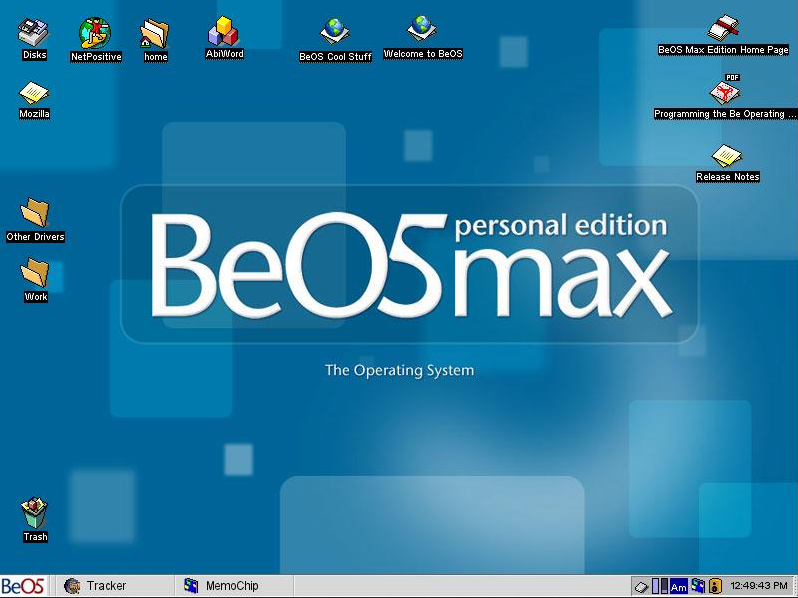
\includegraphics[width=.2\textwidth]{bos}
	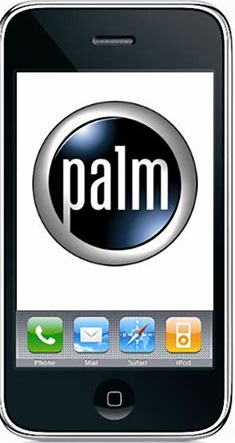
\includegraphics[width=.1\textwidth]{palmos}
	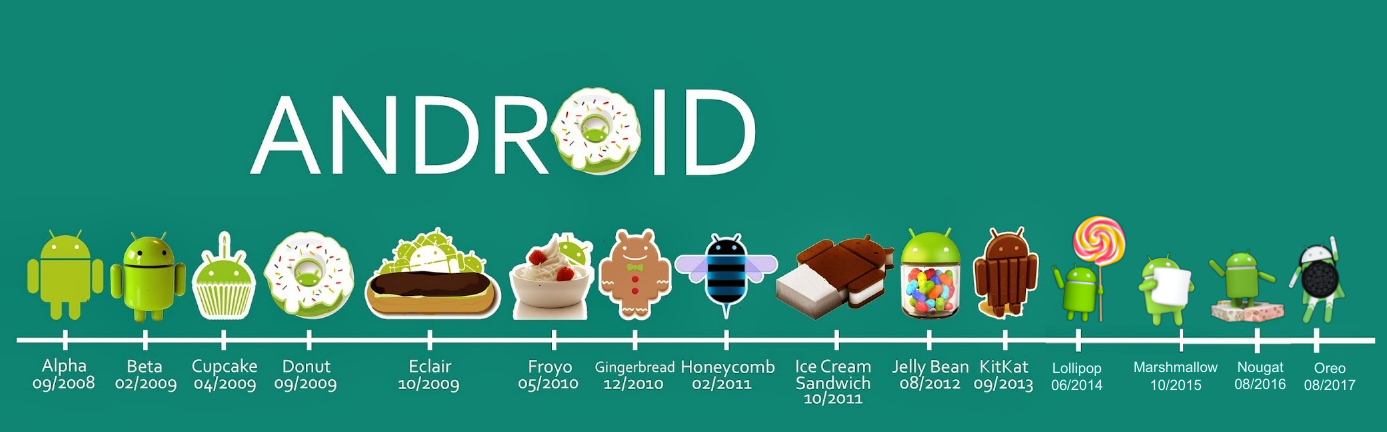
\includegraphics[width=.4\textwidth]{android-history}

	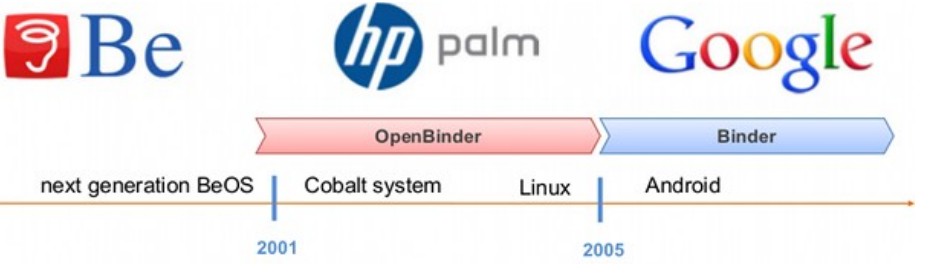
\includegraphics[width=.8\textwidth]{binder-history}
\end{frame}

%----------------------------------------------
\begin{frame}[plain]
	\frametitle{背景介绍}
	\centering
	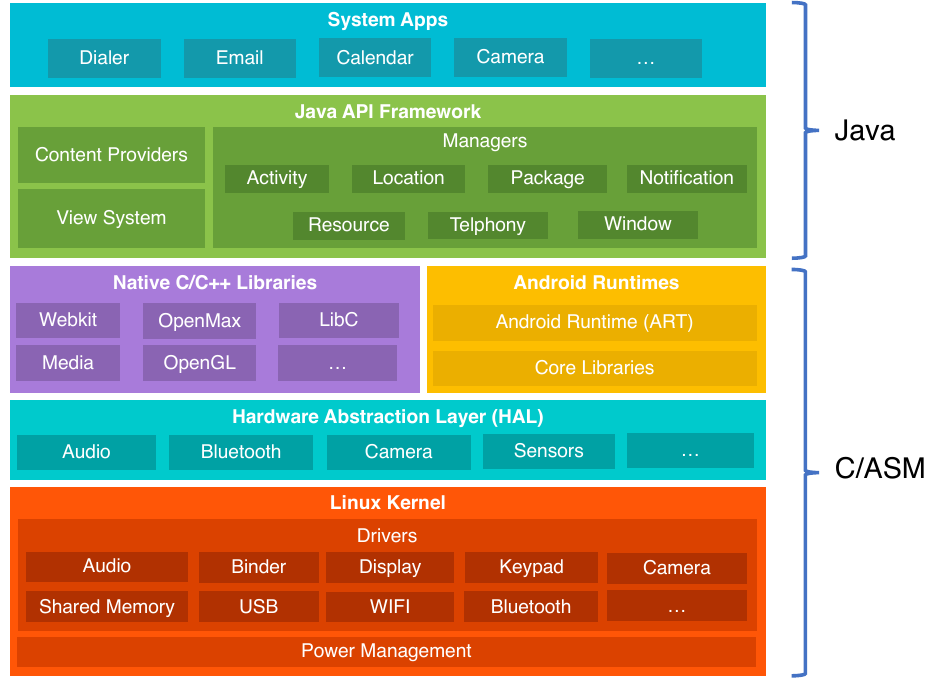
\includegraphics[width=.7\textwidth]{android-arch}
	
\end{frame}
%----------------------------------------------
\begin{frame}[fragile]
	\frametitle{背景介绍}
	%    \framesubtitle{xxxx}
	
	\begin{columns}
		\begin{column}{.4\textwidth}
			
			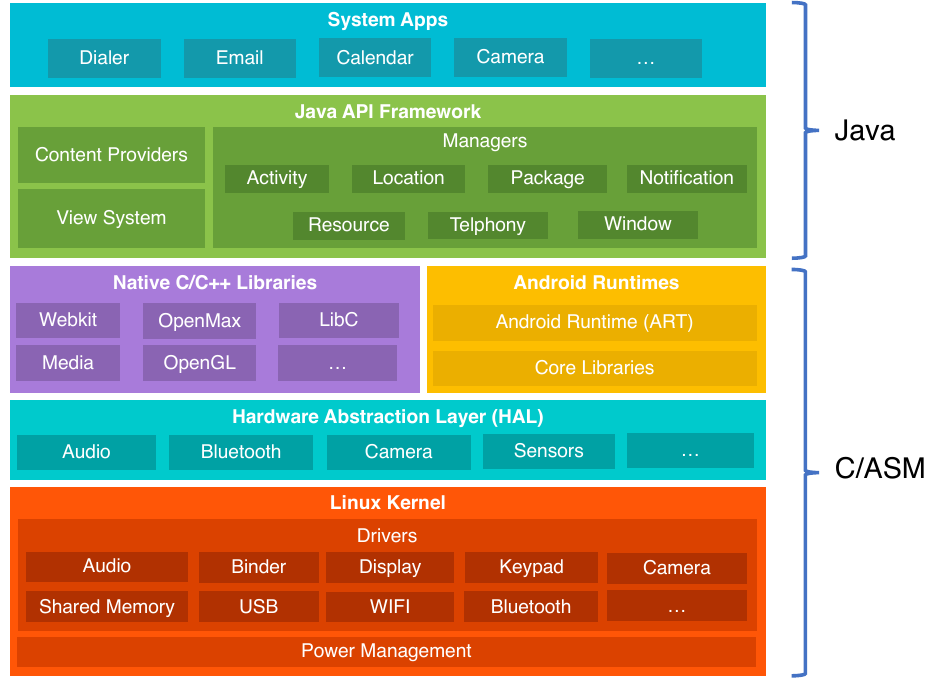
\includegraphics[width=1.\textwidth]{android-arch}
			
		\end{column}
		\begin{column}{.6\textwidth}
			Linux kernel v.s. Android
			\begin{itemize}
				\item binder -- 新的IPC机制
				\item ashmem -- 新的shared memory机制
				\item logger
				\item ......
			\end{itemize}
		
			\begin{block}{Binder: Android's Solution}
			“In the Android platform, the binder is used for
			nearly everything that happens across processes
			in the core platform. " – Dianne Hackborn
			https://lkml.org/lkml/2009/6/25/3
			
		\end{block} 
		\end{column}
	\end{columns}
\end{frame}


%----------------------------------------------
\begin{frame}[fragile]
	\frametitle{背景介绍}
	%    \framesubtitle{xxxx}
	
	\begin{columns}
		\begin{column}{.4\textwidth}
			
			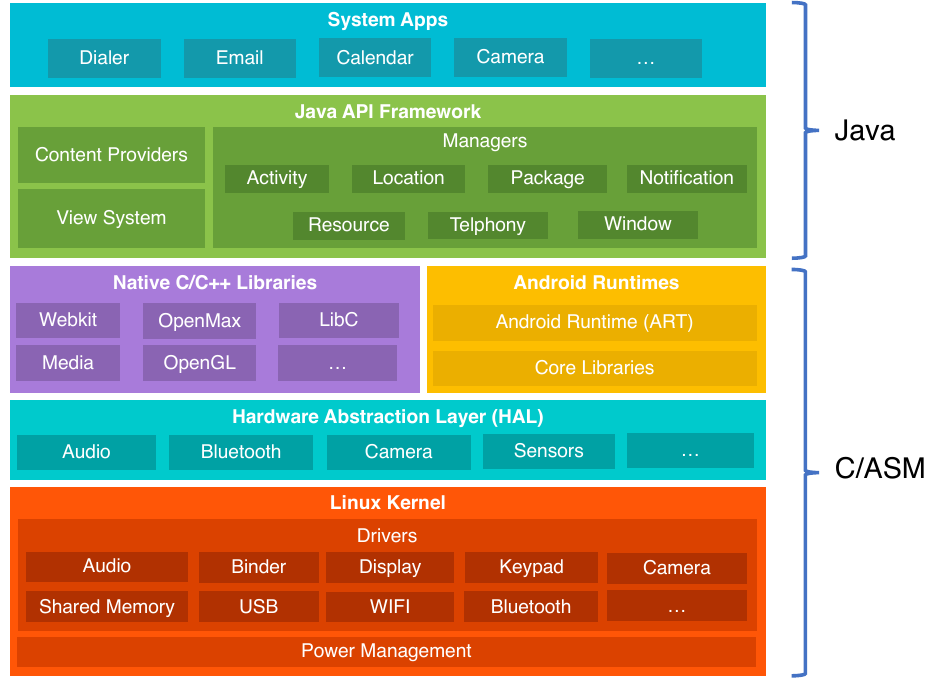
\includegraphics[width=1.\textwidth]{android-arch}
			
		\end{column}
		\begin{column}{.6\textwidth}
			Android进程
			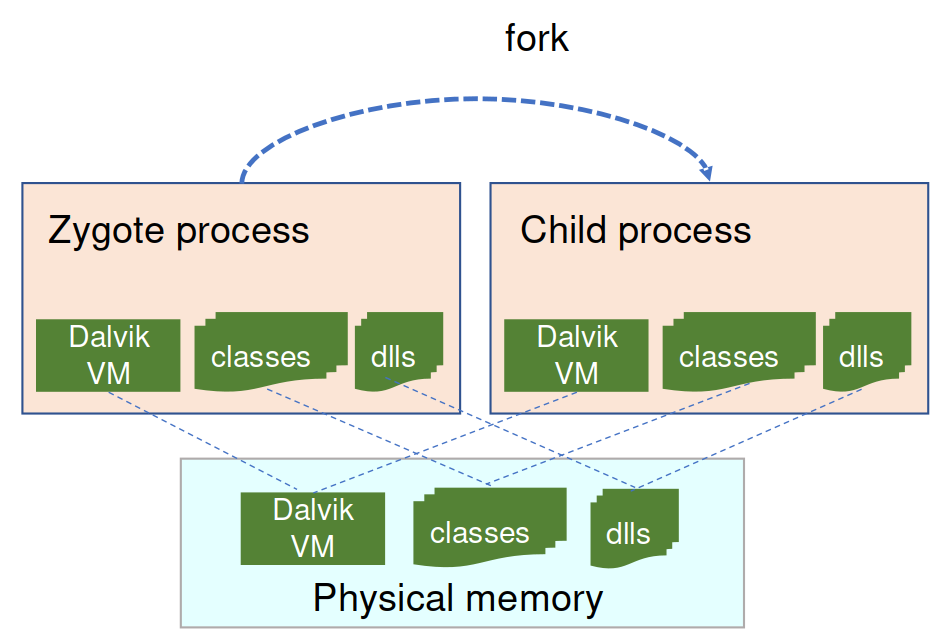
\includegraphics[width=1.\textwidth]{android-fork}

		\end{column}
	\end{columns}
\end{frame}


%----------------------------------------------
\begin{frame}[fragile]
	\frametitle{背景介绍}
	%    \framesubtitle{xxxx}
	
	\begin{columns}
		\begin{column}{.5\textwidth}
			Android进程
			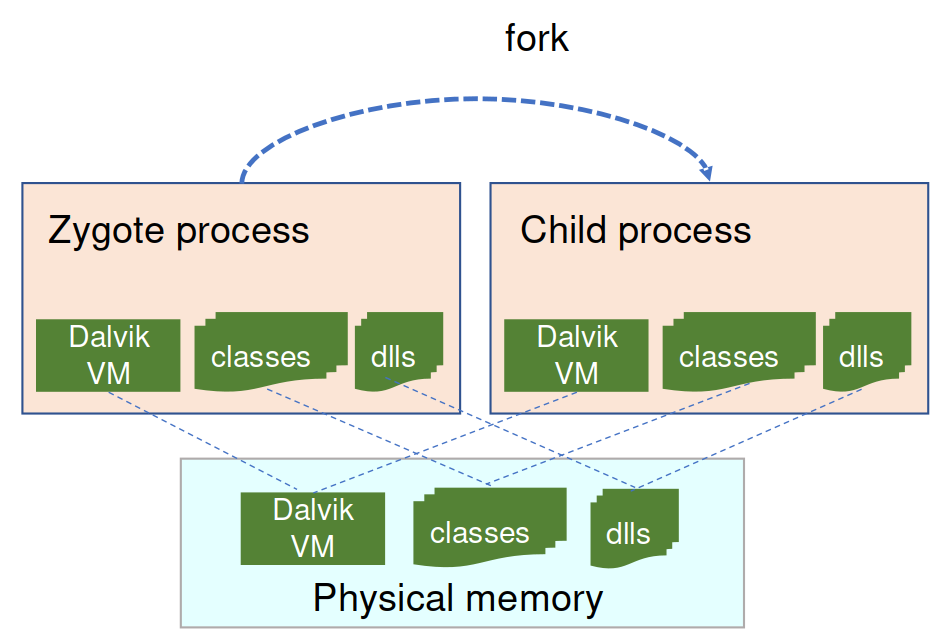
\includegraphics[width=1.\textwidth]{android-fork}
			
		\end{column}
		\begin{column}{.5\textwidth}
			Android任务 task
			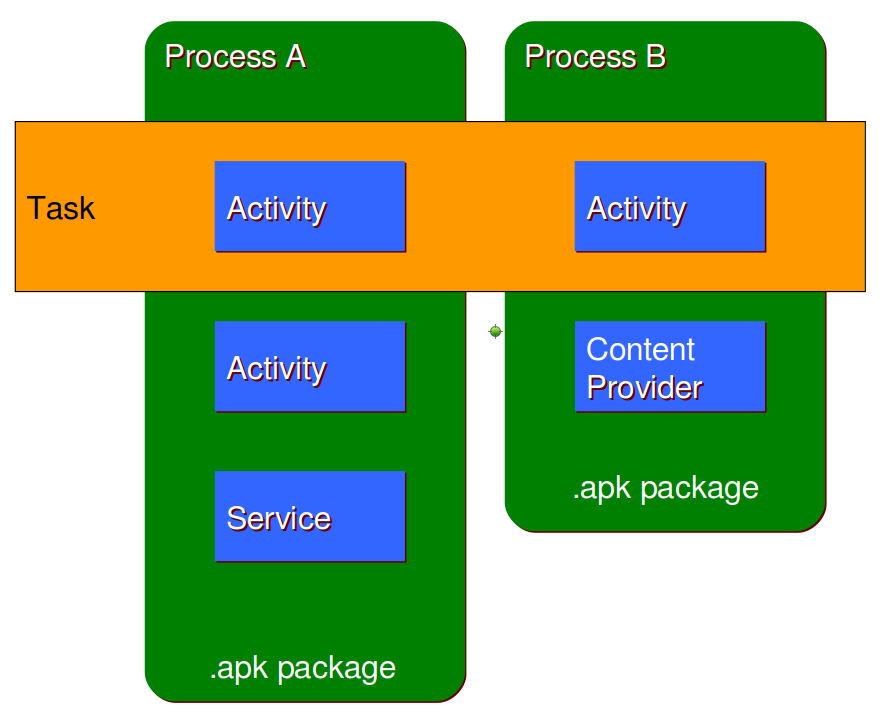
\includegraphics[width=1.\textwidth]{android-task}
			
		\end{column}
	\end{columns}
\end{frame}

%----------------------------------------------
\begin{frame}[fragile]
	\frametitle{背景介绍}
	%    \framesubtitle{xxxx}
	
	\begin{columns}
		\begin{column}{.5\textwidth}
			Android任务task
			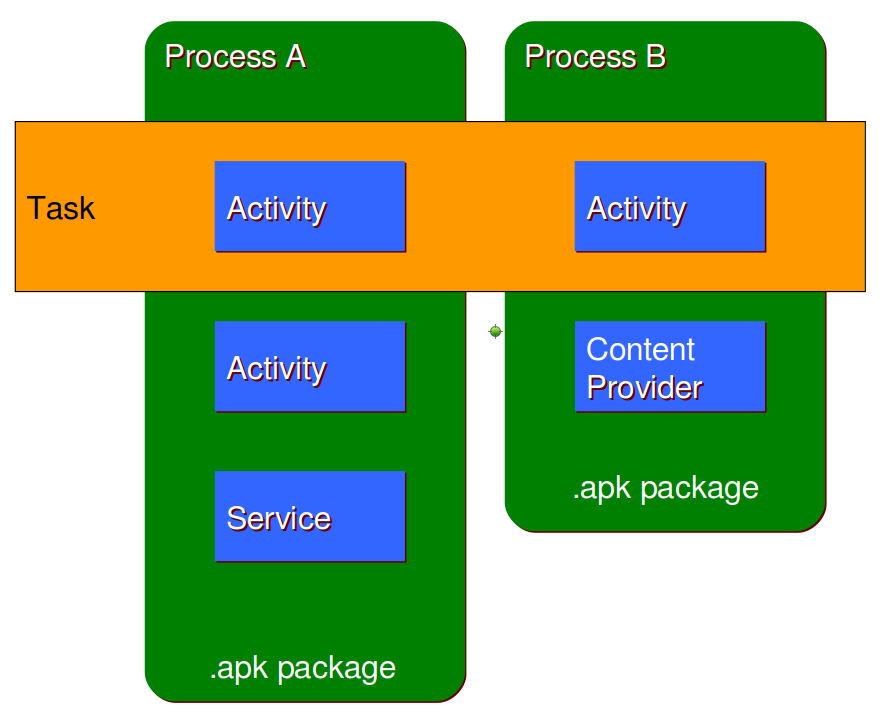
\includegraphics[width=1.\textwidth]{android-task}
			
		\end{column}
		\begin{column}{.5\textwidth}
			Android任务如何跨进程交互?
			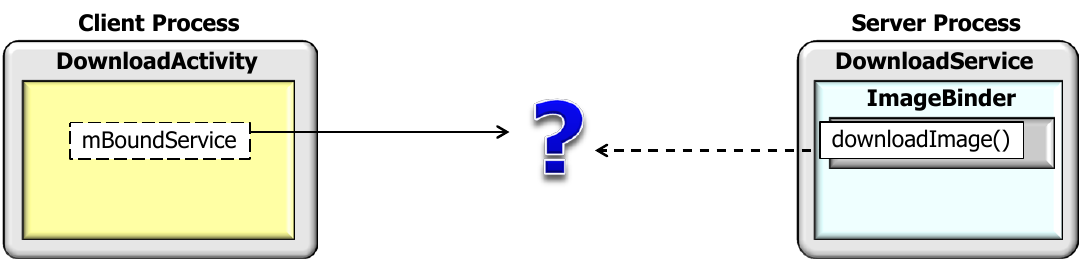
\includegraphics[width=1.\textwidth]{android-how-ipc}
			
		\end{column}
	\end{columns}
\end{frame}


%----------------------------------------------
\begin{frame}[fragile]
	\frametitle{Binder机制}
	
	\begin{columns}
		\begin{column}{.5\textwidth}
			Android任务如何跨进程交互?
			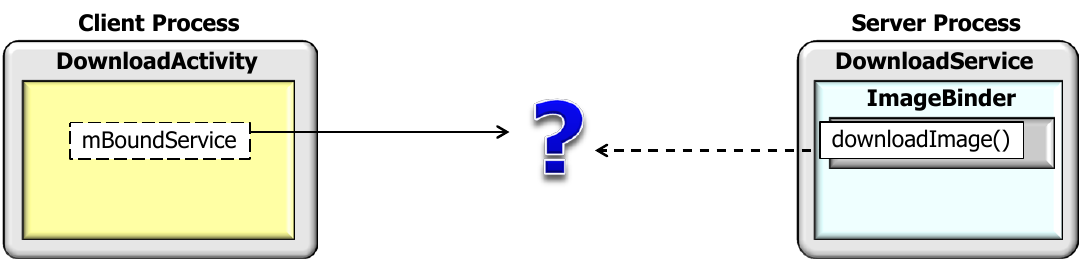
\includegraphics[width=1.\textwidth]{android-how-ipc}
			
		\end{column}
		\begin{column}{.5\textwidth}
			
			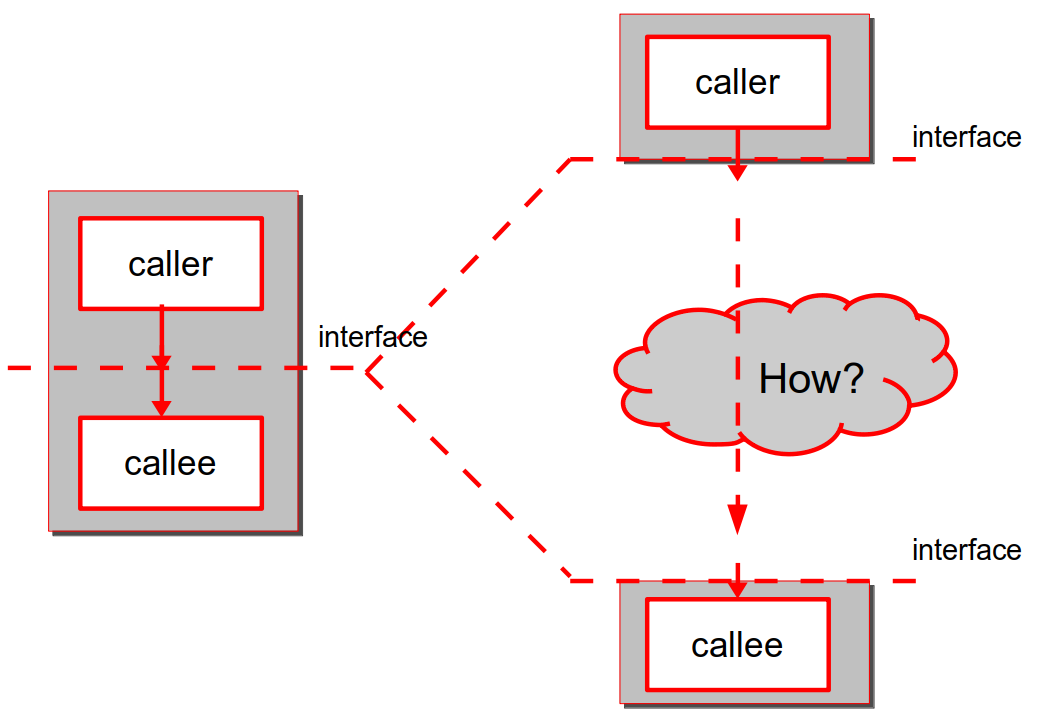
\includegraphics[width=1.\textwidth]{binder-simple1}
			
		\end{column}
	\end{columns}
\end{frame}


%----------------------------------------------
\begin{frame}[fragile]
	\frametitle{Binder机制}
	%    \framesubtitle{xxxx}
	
	\begin{columns}
		\begin{column}{.5\textwidth}
			Android任务如何跨进程交互?
			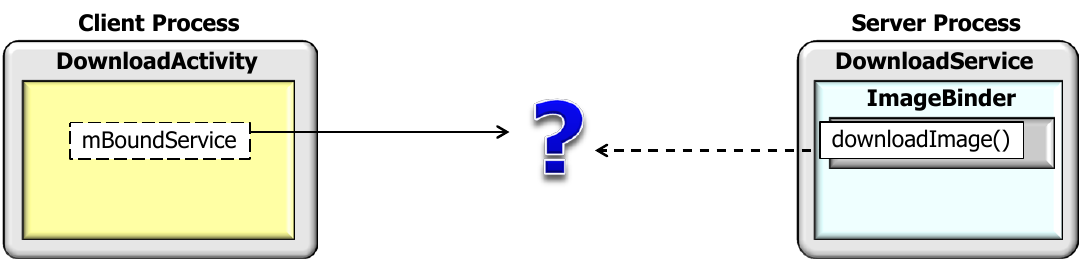
\includegraphics[width=1.\textwidth]{android-how-ipc}
			
		\end{column}
		\begin{column}{.5\textwidth}
			
			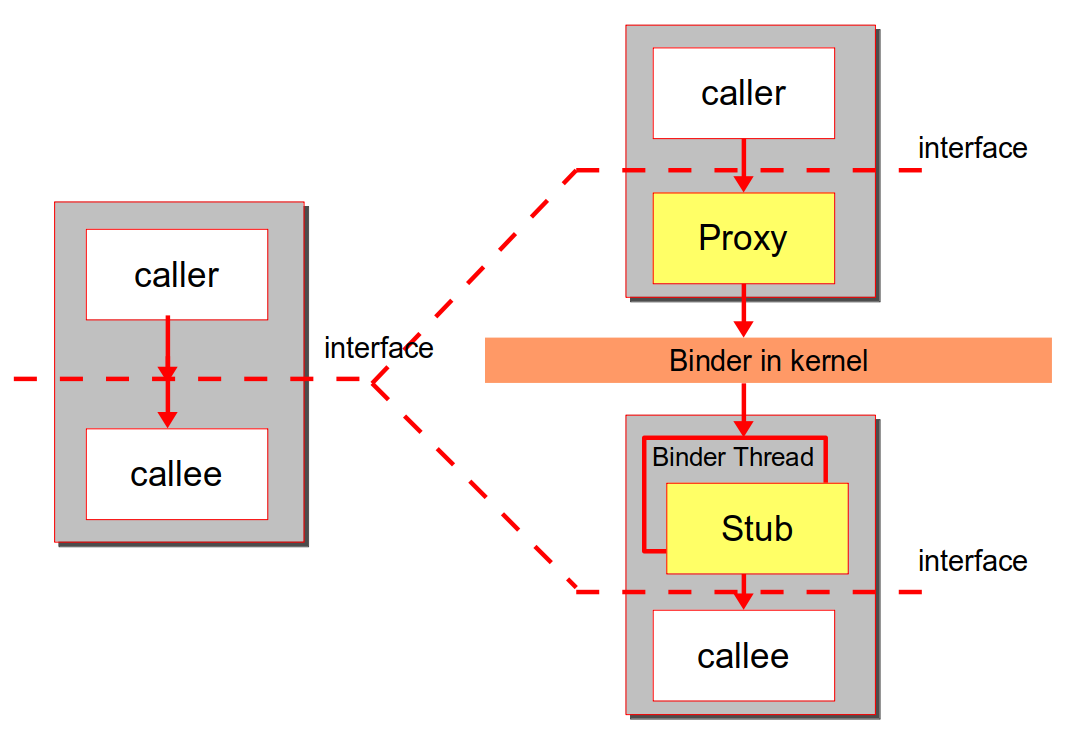
\includegraphics[width=1.\textwidth]{binder-simple2}
			
		\end{column}
	\end{columns}
\end{frame}


%----------------------------------------------
\begin{frame}[fragile]
	\frametitle{Binder机制}
	%    \framesubtitle{xxxx}
	
	\begin{columns}
		\begin{column}{.5\textwidth}
			Android任务如何跨进程交互?
			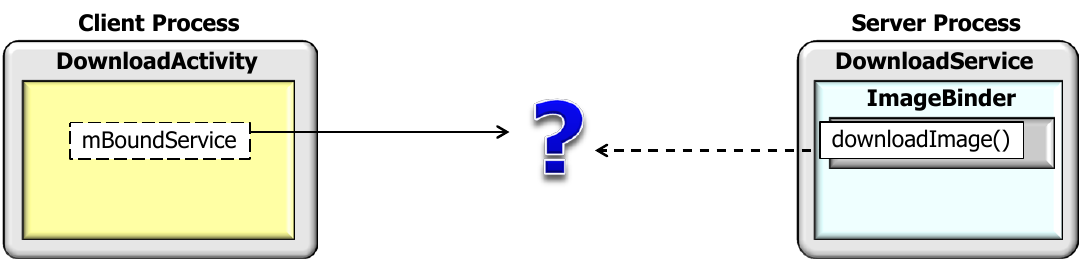
\includegraphics[width=1.\textwidth]{android-how-ipc}
			
		\end{column}
		\begin{column}{.5\textwidth}
			
			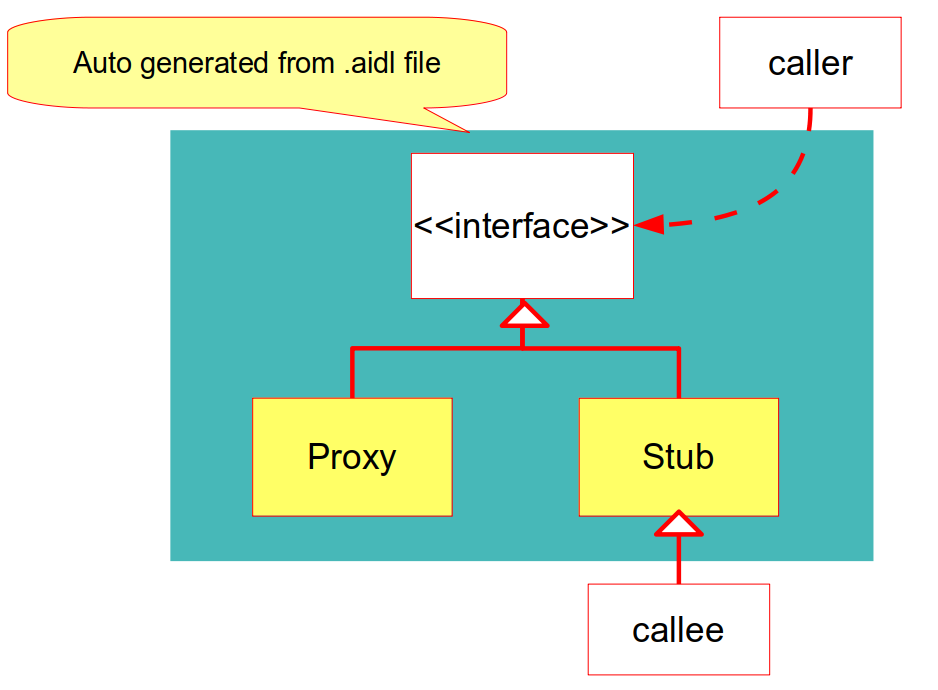
\includegraphics[width=1.\textwidth]{binder-idl}
			
		\end{column}
	\end{columns}
\end{frame}

%----------------------------------------------
\begin{frame}[fragile]
	\frametitle{Binder机制}
	%    \framesubtitle{xxxx}
	
	\begin{columns}
		\begin{column}{.5\textwidth}
%			Android任务如何跨进程交互?
			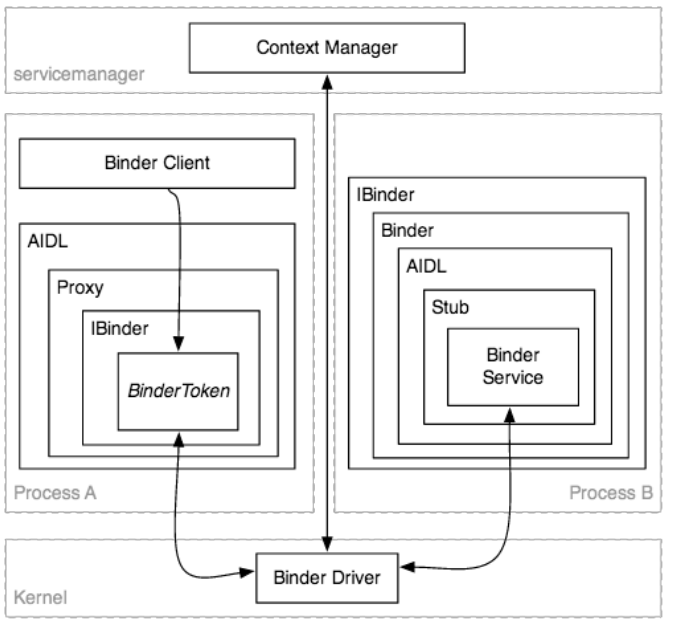
\includegraphics[width=1.\textwidth]{binder-layer}
			
		\end{column}
		\begin{column}{.5\textwidth}
		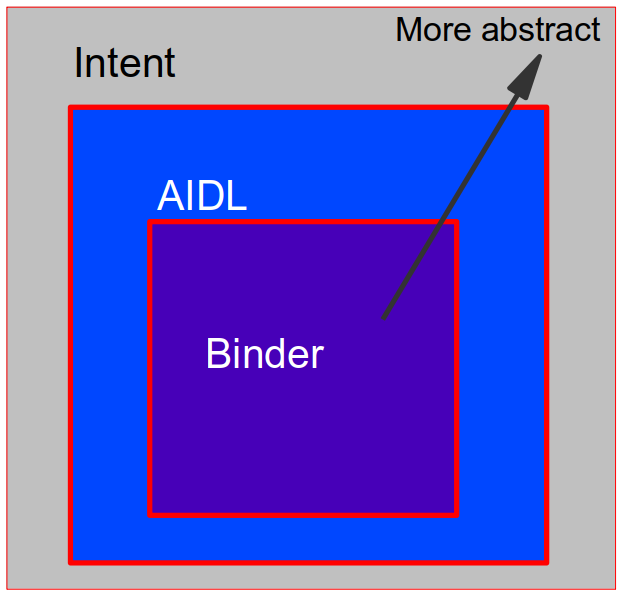
\includegraphics[width=.5\textwidth]{binder-abstract}	
				\begin{itemize}
		\item Intent -- 最高层的IPC抽象
		\item AIDL -- Android Interface Definition Language
		\item binder: kernel driver
		\item ashmem: shared memory
		\end{itemize}
			
		\end{column}
	\end{columns}
\end{frame}
%----------------------------------------------
\begin{frame}[plain]
	\frametitle{Binder机制}
	\centering
	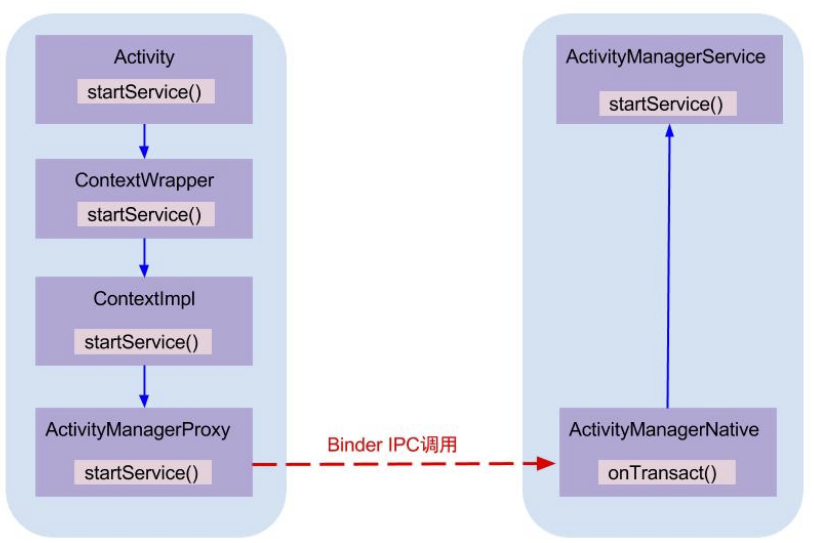
\includegraphics[width=.8\textwidth]{binder-call}
	
\end{frame}

\begin{frame}[plain]
	\frametitle{Binder机制}
%	\centering
%	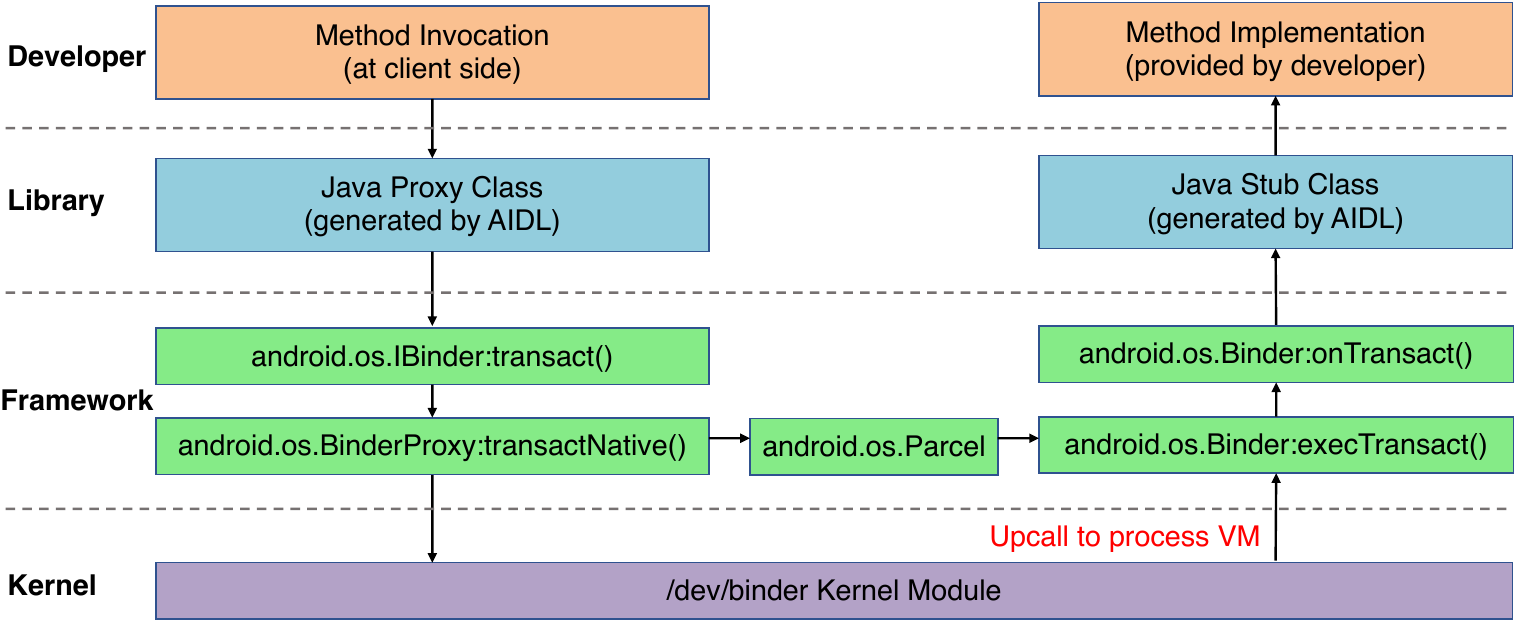
\includegraphics[width=1.\textwidth]{binder-infoflow}
	
	
		\begin{columns}
		\begin{column}{.6\textwidth}

			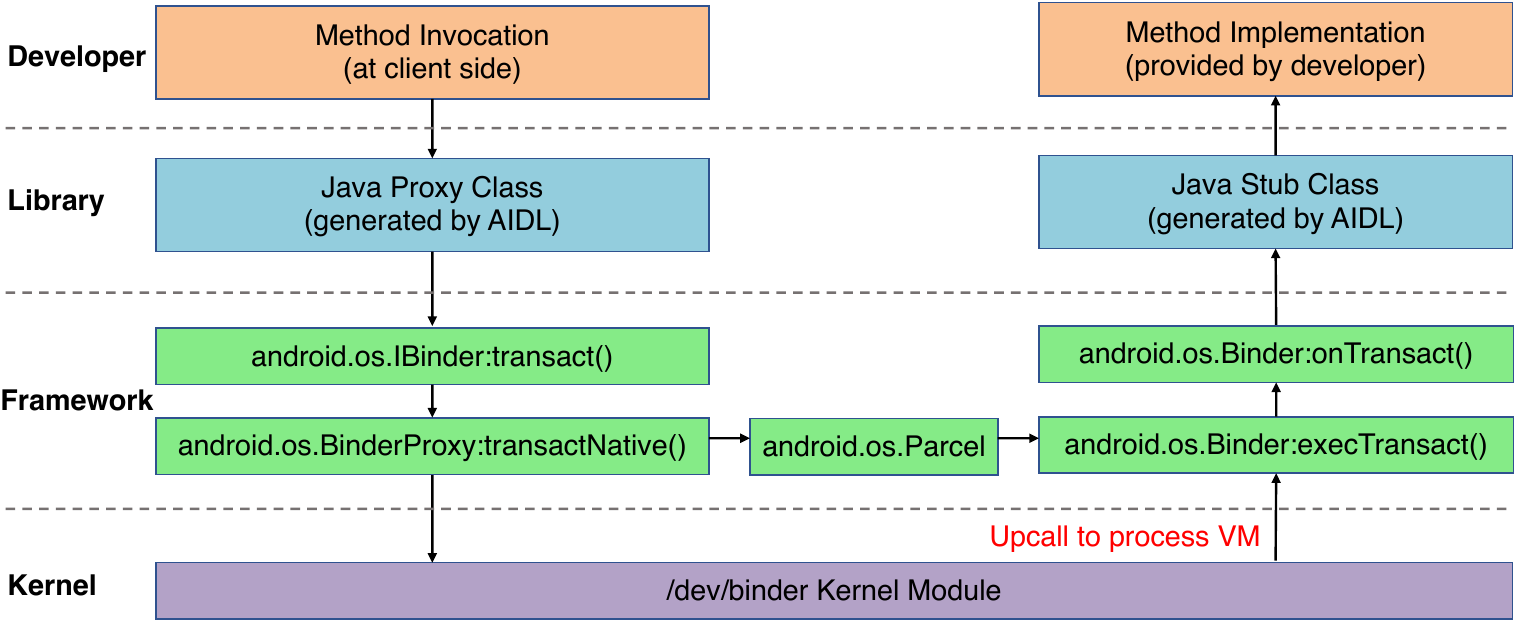
\includegraphics[width=1.\textwidth]{binder-infoflow}
			
		\end{column}
		\begin{column}{.4\textwidth}
			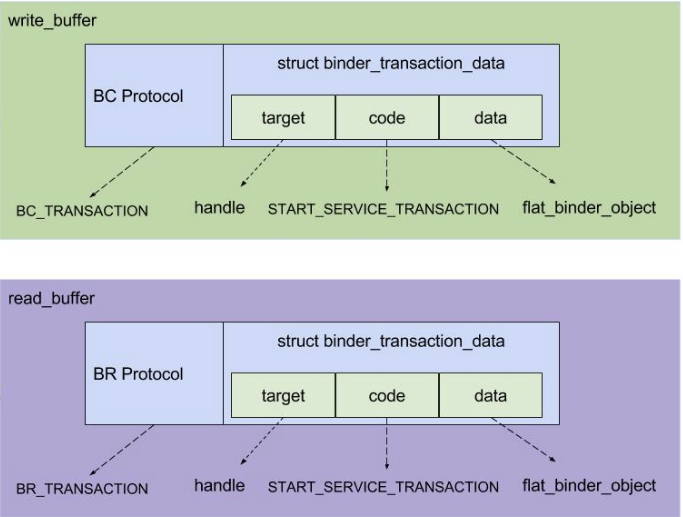
\includegraphics[width=1.\textwidth]{binder-buf}	
%			\begin{itemize}
%				\item Intent -- 最高层的IPC抽象
%				\item AIDL -- Android Interface Definition Language
%				\item binder: kernel driver
%				\item ashmem: shared memory
%			\end{itemize}
			
		\end{column}
	\end{columns}

\end{frame}

\begin{frame}[plain]
	\frametitle{Binder机制}
	\centering
	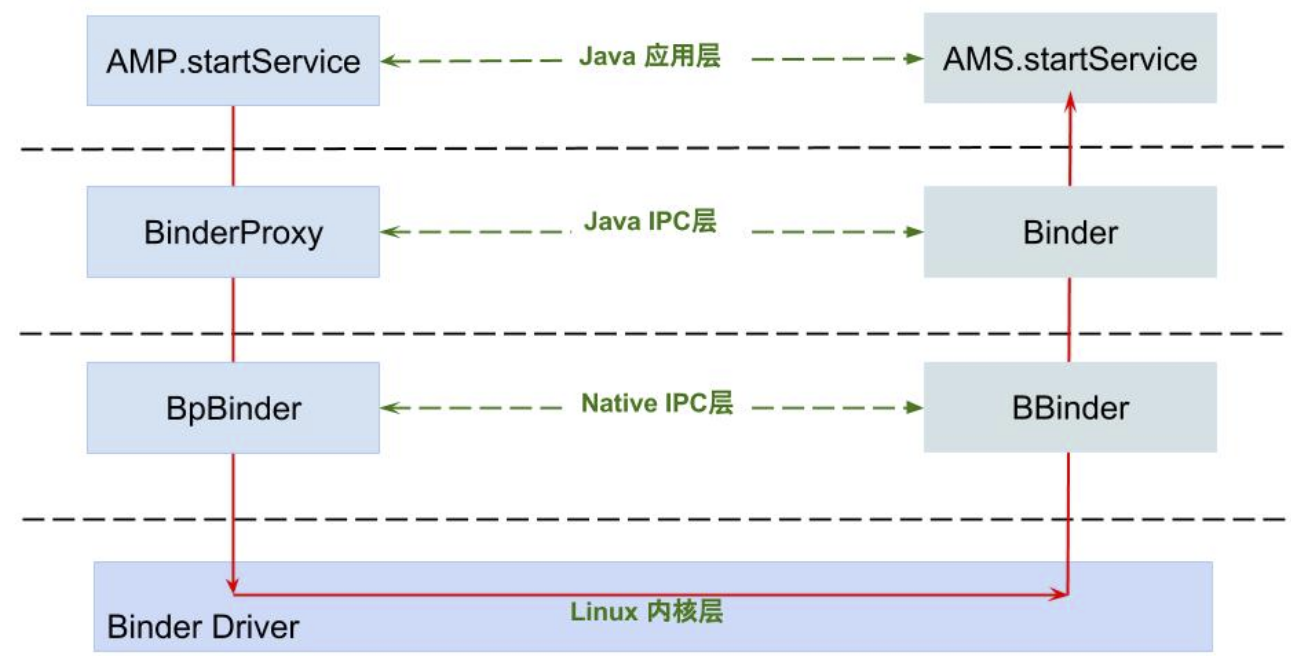
\includegraphics[width=1.\textwidth]{binder-ctr-layers}
	
\end{frame}

\begin{frame}[plain]
	\frametitle{Binder机制}
	\centering
	
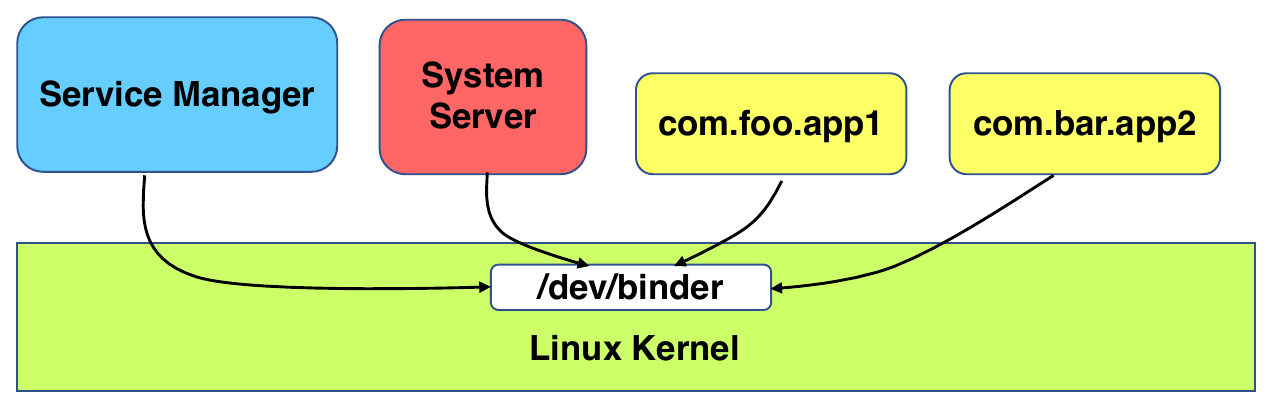
\includegraphics[width=.6\textwidth]{binder-ex1}
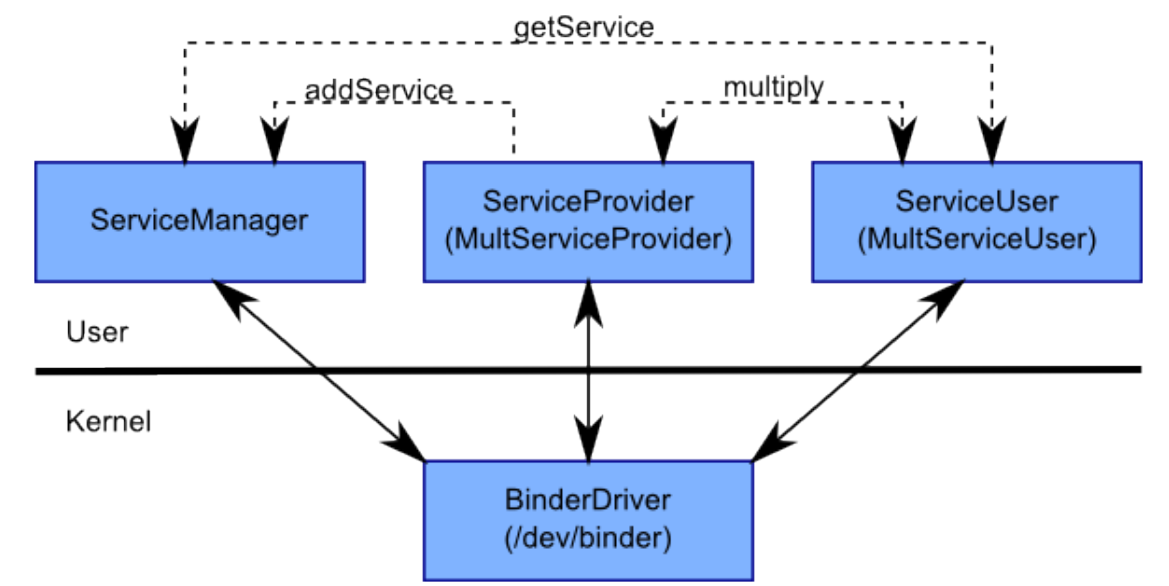
\includegraphics[width=.6\textwidth]{binder-ex3}
	
\end{frame}

%----------------------------------------------
\begin{frame}[plain]
	\frametitle{Binder机制 }
	
	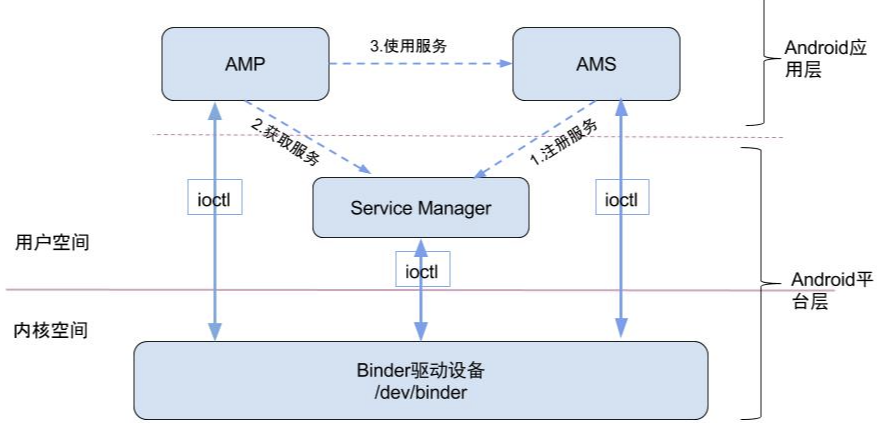
\includegraphics[width=.9\textwidth]{binder-arch-sm}
	
\end{frame}
%-------------------------
%----------------------------------------------
\begin{frame}[plain]
	\frametitle{Binder机制 -- 一次拷贝}

	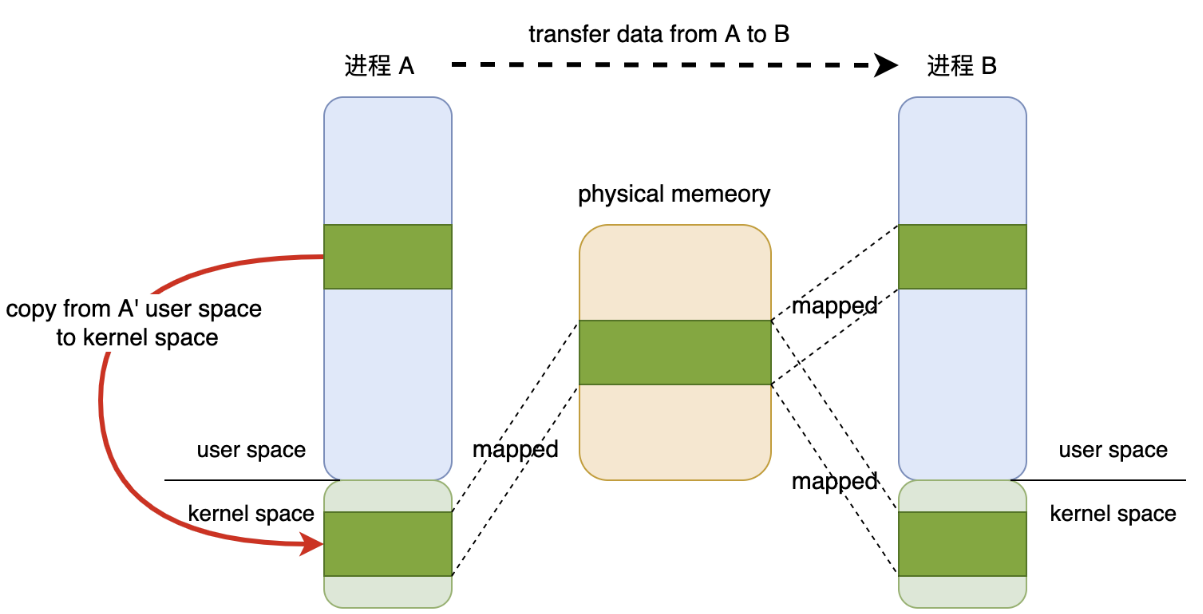
\includegraphics[width=1.\textwidth]{binder-one-copy}

\end{frame}

%----------------------------------------------
\begin{frame}[plain]
	\frametitle{参考}
	
			\begin{itemize}
				\item \href{http://www.dre.vanderbilt.edu/~schmidt/cs282/PDFs/android-binder-ipc.pdf}{Android IPC Mechanism}, Jim Huang (黄敬群), 2012
				\item \href{https://www.cs.jhu.edu/~huang/cs318/fall18/lectures/lec20_mobile_ds.pdf}{Lec20}: CS 318 Principles of Operating Systems, Ryan Huang, 2020			
				\item \href{https://events.static.linuxfound.org/images/stories/slides/abs2013_gargentas.pdf}{Deep Dive into Android IPC/Binder Framework at Android Builders Summit}, Aleksandar Gargenta, 2013				
				\item \href{http://gityuan.com/2016/09/04/binder-start-service/}{彻底理解Android Binder通信架构}, Gityuan, 2016
			\end{itemize}
	
\end{frame}
%----------------------------------------------
%----------------------------------------------
\end{document}
